%\section{HDMI}
%\subsection{Implementation}
For the first prototypes of the project VGA was used to stream the images to a screen. That needed to be changed because of two reasons: Firstly digital visual interfaces can get provide better resolution than analogue ones and secondly, and that is the actual main reason, the atlys board does not have a VGA port.

\subsubsection{HDMI - Principle of Operation}
HDMI(High Definition Multimedia Interface) is a digital interface which transport visual as well as audio data differential. The used encoding is the same as DVI called Transition-minimized differential signaling. TMDS is a kind of 8b/10b encoding but not the actual 8b/10b used by PCIE. It is optimized to create as less as possible transitions. Fast transitions are the main cause for electromagnetic interference which couples the twisted pair connection. \newline
The TMDS encoder transforms the actual bits with the previous bits with a XOR or a XNOR function. It takes always the one which causes less transitions. This transformation happens for the 8 data bits while the ninth bit encodes which operation was used. Additionally the sustained average DC level should stay similar. Therefore the encoder can invert the data to even out the balance of ones and zeros. This is saved in the tenth bit. \newline
Because of the fact that a HDMI connector just have 19 Pins, the data is transferred sequentially at a higher clockspeed. The first 12 Pins are for the data and the clock. For each color(RGB) and the clock there is a differential pair with one shield connection. That means that the bits have to be transferred with a 10 times faster clock than the clock which generates the pixel.



\subsubsection{HDMI with Spartan6 FPGAs on Atlys Boards}
The Atlys Board which is used in the project got 4 HDMI ports. The one which is called J2 is a usual Type A HDMI Connector. With this information it is possible to get the right constraints out of the following table(\ref{hdmi_constraints}).

\begin{figure}[h!]
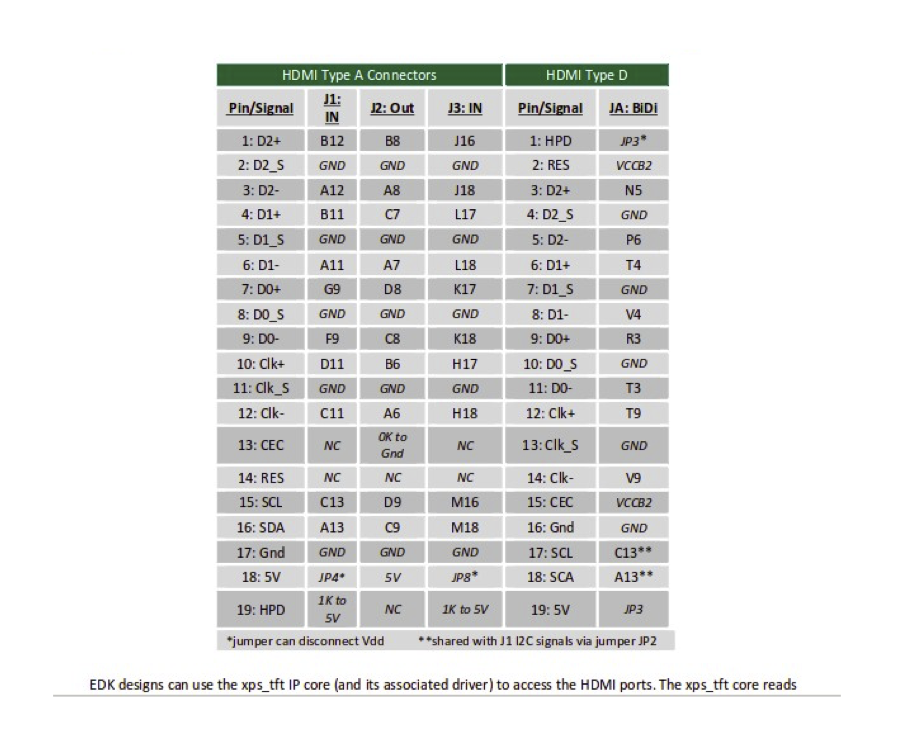
\includegraphics[scale=1.1]{images/hdmi_constraints.png} 

\caption{Constraints for HDMI(out of the Atlys User Manual)}
\label{hdmi_constraints}
\end{figure}

The actual design for the HDMI interface is shown in \ref{hdmi_design}. 
\begin{figure}[h!]
	\centering
	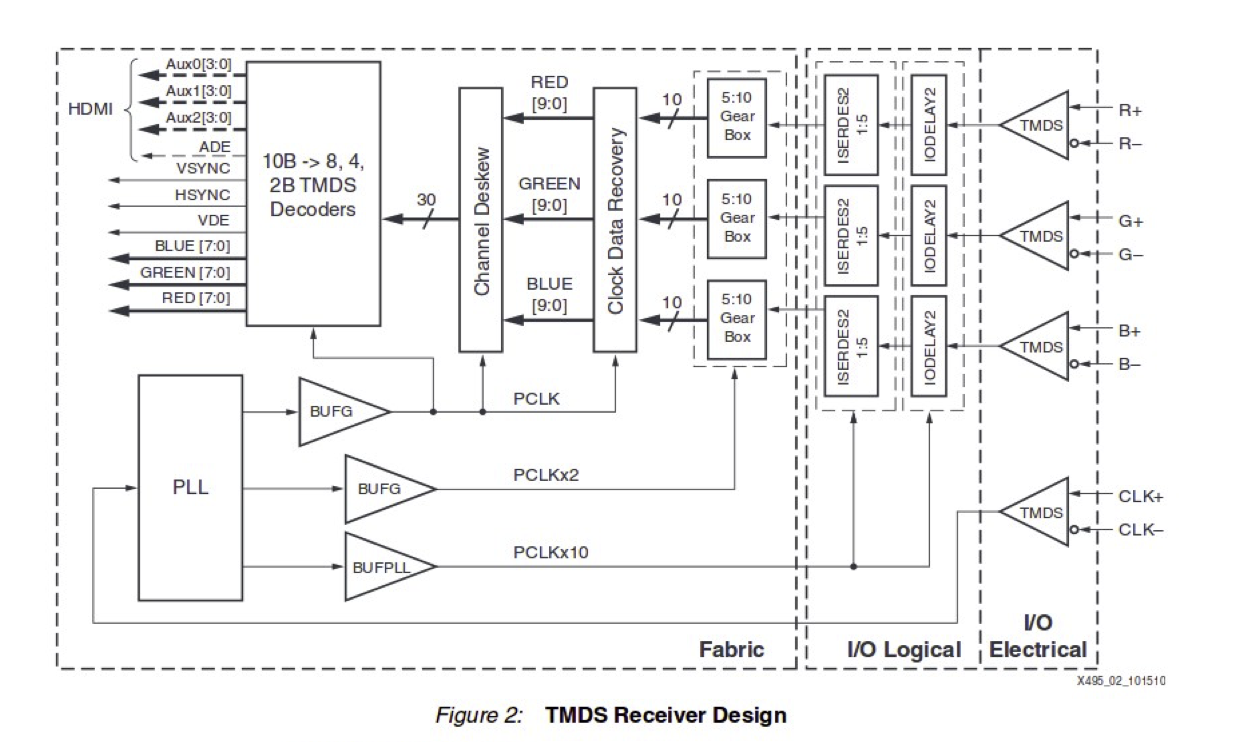
\includegraphics[scale=0.7]{images/hdmi_design.png}

\caption{Design how to build a HDMI interface(out of the TMDS User Interface Manual for Spartan6)}
\label{hdmi_design}
\end{figure}
This is a reference design by Xilinx itself. In the presented design the audio HDMI interface was not used, so ignore this part. Because of that there are just the video signals and the pixel clock there to mention. At first the RGB data is encoded by the TMDS module like it was described in the sections before. For a well synchronized transfer we need at the same time a perfectly timed pixel clock at a speed of 74.25 MHz. Because 74.25 MHz is hard to reach out of 100 MHz, 75 MHz were taken and it still worked fine. This clock was needed to be created by the clockwizard IP. In the next parts the TMDS encoded RGB data is converted and serialized into the differential TMDS signals. Because of the serialization we need a 10 times faster clock which is created out of the PLL shown in the schematic. Additionally to RGB data the clock is sent as well for synchronization.

